%% \chapter{Properties and flavours \Author{P. Brisk}\\\progressbar[0.4\textwidth]{writing}{80}}
\chapter{Properties and flavours \Author{P. Brisk}}
\inputprogress
\label{chap:properties_and_flavours}


\section{Preliminaries}

Recall from the previous chapter that a procedure is in SSA Form if it
every variable is defined once, and every use of a variable corresponds
to exactly one definition. Many variations, or flavors, of SSA Form that 
satisfy these criteria can be defined, each offering its own considerations.
For example, different flavors vary in terms of the number of $\phi$-functions,
which affects the size of the intermediate representation; some are more difficult to construct, maintain, and destruct
compared to others. This chapter explores these SSA flavors and provides
insight onto the contexts that favor some over others. 

\section{Def-Use and Use-Def Chains}
Under SSA Form, each variable is defined once. Def-use chains are data structures that provide for the single definition of a variable the set of all its uses. Each use-def chain inversely provides for each use of a variable its unique definition. As we will illustrate further in the book (see~Chapter~\ref{chapter:propagation_engine}) def-use chains are useful for forward data-flow analysis as they provide direct connections that shorten the propagation distance between nodes that generate and use data-flow information. 

Because of its single definition per variable property, SSA form simplifies def-use and use-def chains in several ways. First, SSA form simplifies def-use chains as it combines the information as early as possible.
This is illustrated by Figure~\ref{fig:properties_and_flavors:du} where the def-use chains in the non-SSA program requires as many merge as $x$ is used while the corresponding SSA form allows early and more efficient combination. 

Second, as it is easy to associate to each variable its single defining operation, use-def chains can be explicitly represented and maintained almost for free. As this constitutes the skeleton of the so called SSA graph (see Chapter~\ref{chap:vsdg}), when considering a program under SSA form, use-def chains are implicitly considered as a given. 
The explicit representation of use-def chains simplifies backward 
propagation, which favors algorithms such as dead-code elimination. 

For forward propagation, def-use chains being just the reverse of use-def chains, computing it is also easy, and maintaining it can be done without much efforts either. 
However, even without def-use chains, some lightweight forward propagation algorithms such as copy-folding are possible and show to be already quite efficient using only use-def chains: if loops are conservatively ignored, operations can be processed in topological order so that many definitions are processed prior to the uses. 


\begin{figure}
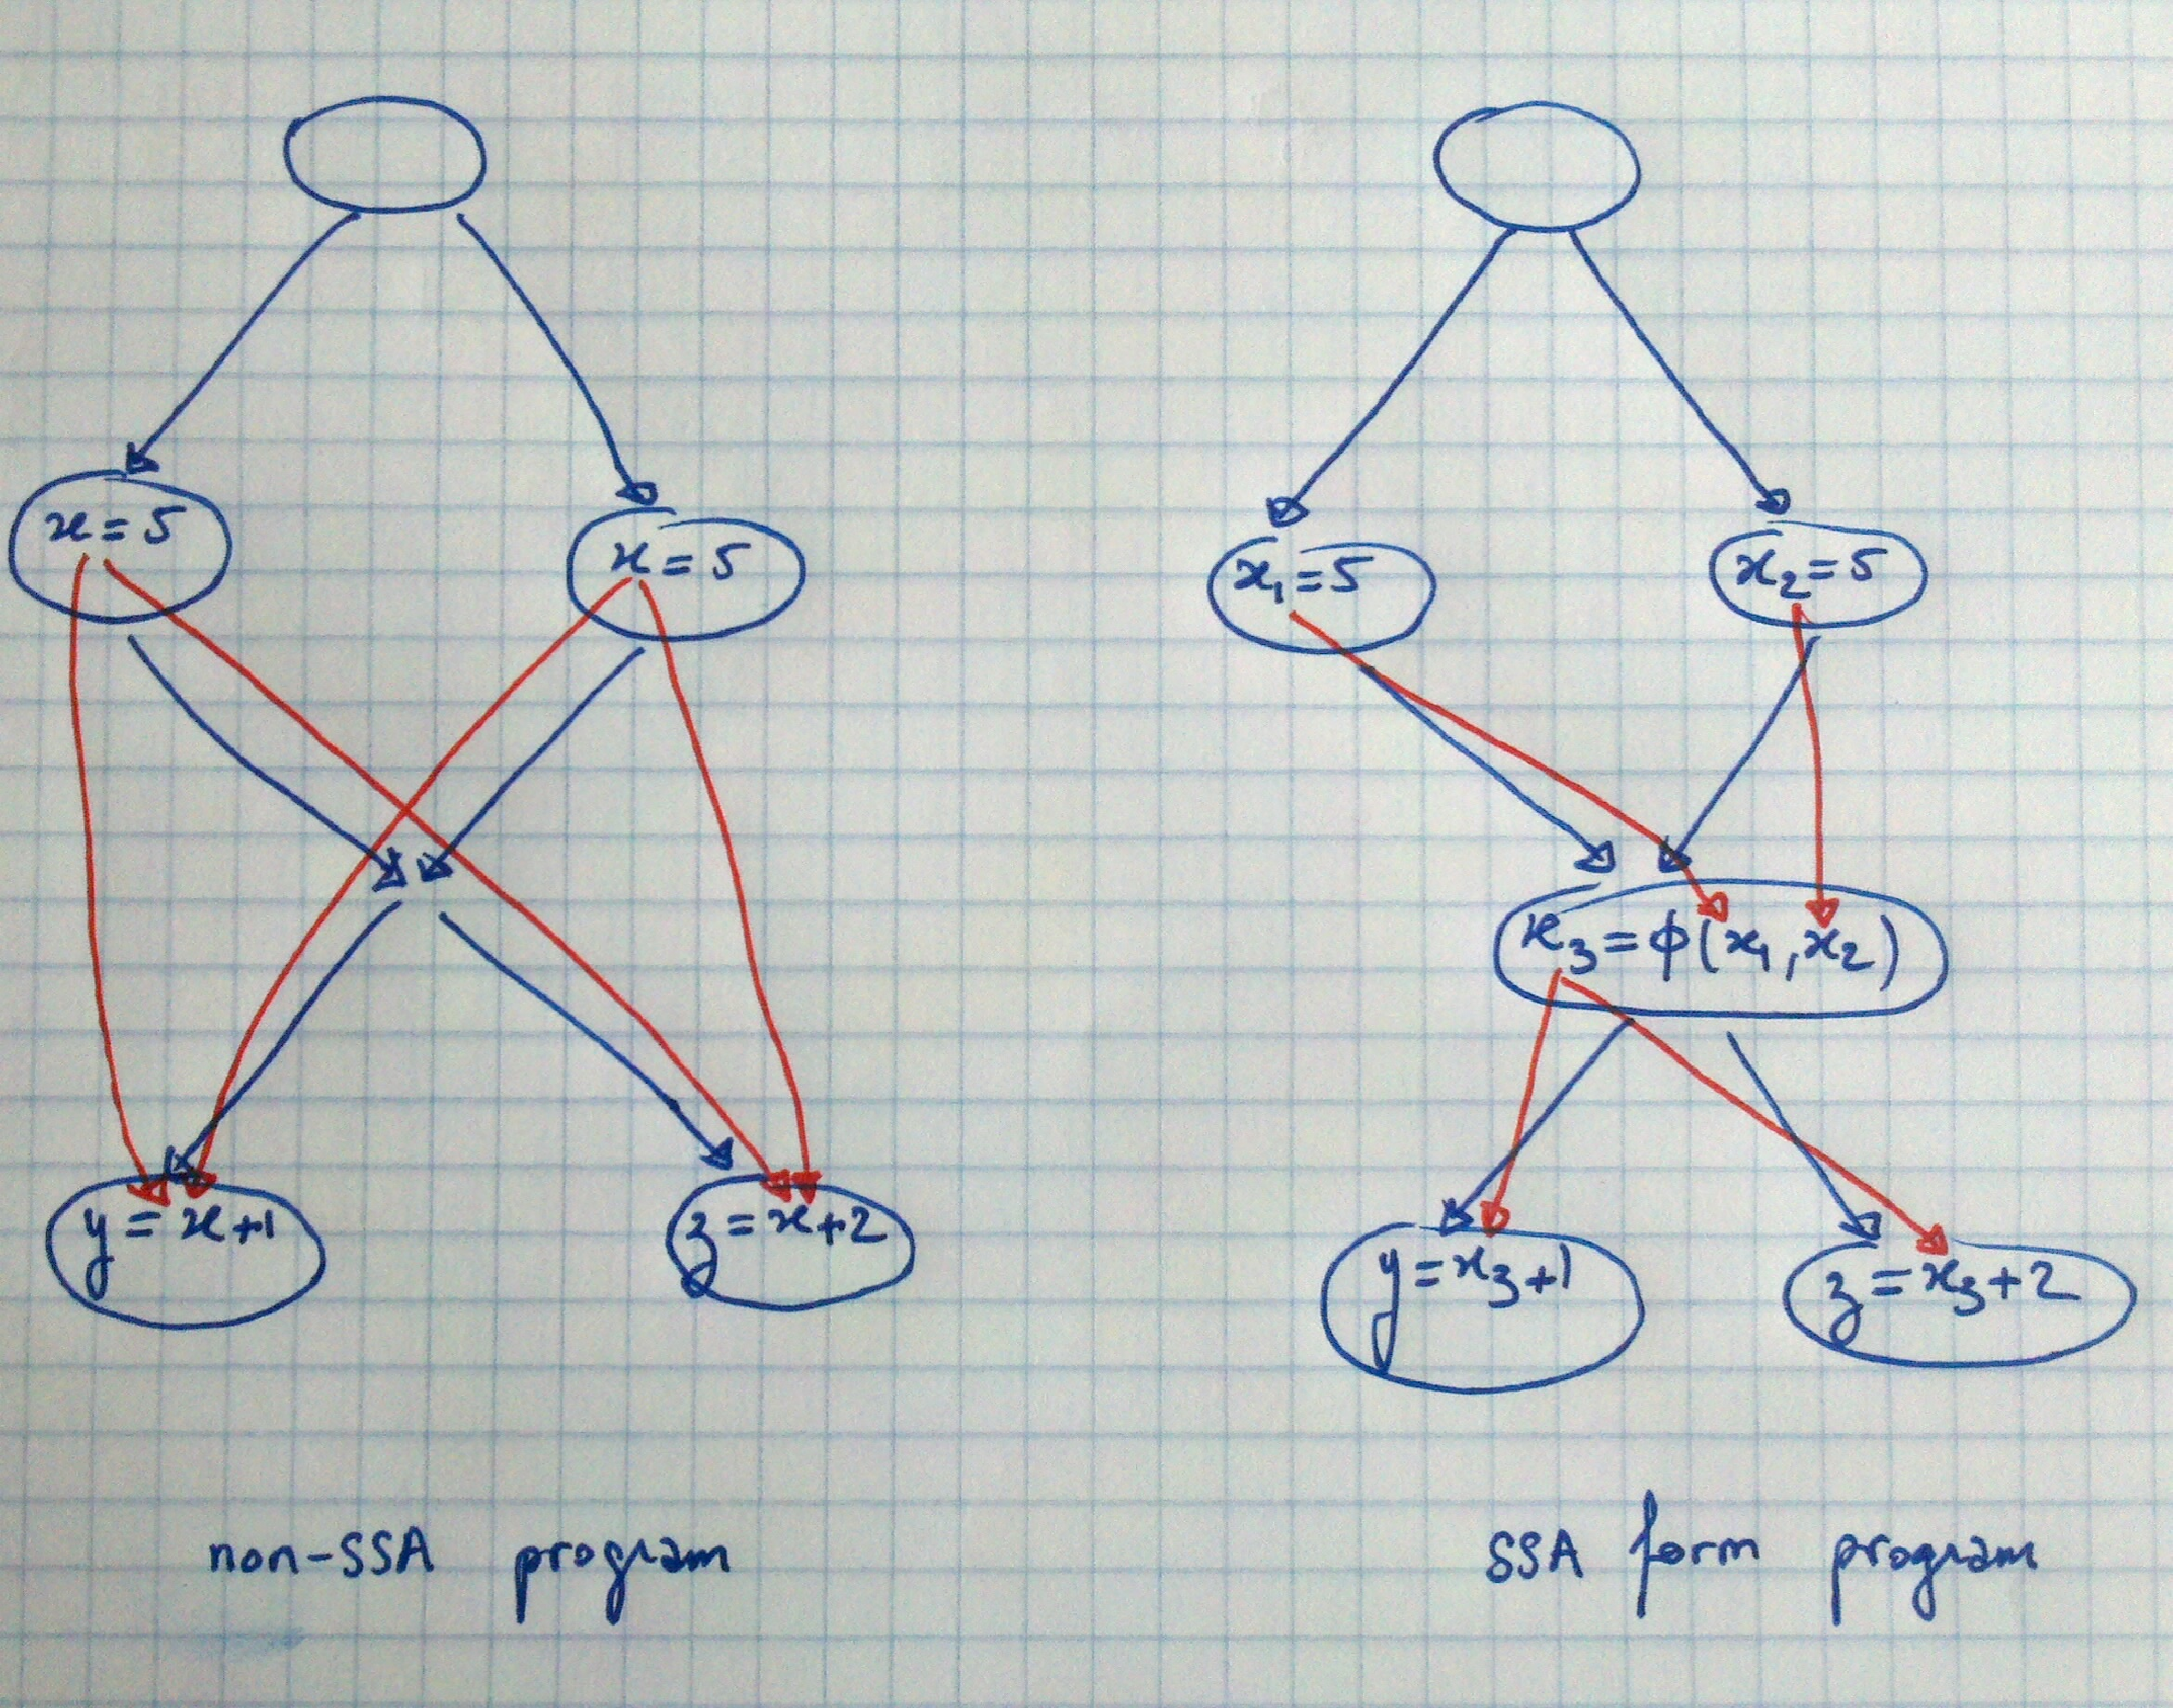
\includegraphics[width=0.7\textwidth]{du.pdf}
\caption{\label{fig:properties_and_flavors:du} Def-use chains (in red) for non-SSA form and its corresponding SSA form program} 
\end{figure}



\section{Minimality}
\label{sec:properties_and_flavors:minimality}

SSA construction is a two-phase process: placement of $\phi$-functions,
followed by renaming. The goal of the first phase is to generate a code that fulfills the further defined single reaching-definition property. Minimality is an additional property of the code with 
$\phi$-functions inserted, but prior to renaming; Chapter~\ref{chap:classical_construction_algorithm} describes the classical SSA
construction algorithm in detail, while this section focuses
primarily on describing the minimality property.  

A definition $D$ of variable $v$ \emph{reaches} a point $p$ in the CFG
if there exists a path from $D$ to $p$ that does not pass through another
definition of $v$. We say that a code has the \emph{single reaching-definition property} iff no program point can be reached by two definitions of the same variable. 
Under the assumption that the single reaching-definition property is fulfilled, the \emph{minimality property} states the minimality of the number of inserted $\phi$-functions.

This property can be characterized using the notion of join sets that we introduce next.
Let $n_{1}$ and $n_{2}$ be distinct basic blocks in a CFG. A basic block
$n_{3}$, which may or may not be distinct from $n_{1}$ or $n_{2}$, is 
a \emph{join node} of $n_{1}$ and $n_{2}$ if there exist at least two
non-empty paths, i.e., paths containing at least one CFG edge, from 
$n_{1}$ to $n_{3}$ and from $n_{2}$ to $n_{3}$, respectively, such that
$n_{3}$ is the only basic block that occurs on both of the paths. In
other words, the two paths converge at $n_{3}$ and no other CFG node. 
Given a set $S$ of basic blocks, $n_{3}$ is a join node of $S$ if it
is the join node of at least two basic blocks in $S$. The set of join
nodes of set $S$ is denoted by the set $\J(S)$. 

Intuitively, a join set corresponds to the placement of $\phi$-functions.
In other words, if $n_{1}$ and $n_{2}$ are basic blocks that both
contain the definition of a variable $v$, then we ought to instantiate
$\phi$-functions for $v$ at every basic block in $\J(n_{1}, n_{2})$. 
Generalizing this statement, if $D_v$ is the set of basic blocks containing
definitions of $v$, then $\phi$-functions should be instantiated in
every basic block in $\J(D_v)$. As inserted $\phi$-functions are themselves 
definition points, some new $\phi$-functions should be inserted at $\J(D_v\cup\J(D_v))$. 
Actually it turns out that $\J(S\cup\J(S))=\J(S)$ so the join set of the set of definition points of a variable characterizes exactly the minimum set of program points where $\phi$-functions should be inserted.

We are not aware of any optimizations that require a strict enforcement of minimality property.
However, placing $\phi$-functions only at the join sets can be done easily using a simple topological traversal of the CFG as described in Section~\ref{section:alternative_ssa_construction_algorithms:loop}. Classical techniques place $\phi$-functions of a variable $v$ at $\J(D_v,r)$, with $r$ the entry node of the CFG. There are good reasons for that as we will explain further. Finally, as explained in Section~\ref{section:classical_construction_algorithm:turning} for reducible flow graphs, some copy-propagation engine can easily turn a non-minimal SSA code into a minimal one.

\section{SSA Form with the Dominance Property}
\label{sec-prop-dominance}
%% ; we assume that the CFG entry node includes a 
%% pseudo-definition of every variable in the procedure. Some languages
%% permit the pseudo-definition of a $v$ reaches a use $U$ of $v$; if this
%% path is taken through the CFG, then $v$ will be used without ever
%% being assigned a value. Although this may be permissible in
%% some cases, it is usually indicative of a programmer error or
%% poor software design. 

In a CFG, basic block $n_{1}$ \emph{dominates} basic block $n_{2}$
if every path in the CFG from the entry point to $n_{2}$ includes
$n_{1}$. By convention, every basic block in a CFG dominates itself. Basic 
block $n_{1}$ \emph{strictly dominates} $n_{2}$ if $n_{1}$ dominates
$n_{2}$ and $n_{1} \neq n_{2}$. We use the symbols $n_{1} dom n_{2}$
and $n_{1} sdom n_{2}$ to denote dominance and strict dominance 
respectively.

The minimality property discussed previously mandates that each
program point be reachable by exactly one definition (or pseudo-definition)
of each variable. If a program point $U$ is a use of variable $v$, then the
reaching definition $D$ of $v$ will dominate $U$; otherwise, there is a path
from the CFG entry node to $U$ that does not include $D$, which contradicts
the Minimality Property. If such a  path existed, then the program would not
be in SSA Form, and a $\phi$-function would need to be inserted somewhere
in $DF^{+}(D)$.  

A procedure is defined to be \emph{strict} if every variable
is defined before it is used along every path from the entry
to exit point~\cite{BudimlicJun02}; otherwise, it is \emph{non-strict}. 
Some languages, such as Java, impose strictness as part of the language
definition; others, such as C/C++, impose no such restrictions. 
 
Adding a pseudo-definition of each variable to the procedure's entry
point ensures strictness. After $\phi$-functions have been placed
for each variable in the program, the presence of the pseudo-definition
as a parameter of a $\phi$-function indicates a potential problem with
an uninitialized variable, as illustrated by the following example:

(Fabrice: Please insert a print-quality version of the figure
"dom\_property.jpeg" which is a scan of a handwritten note. The
content of the figure is correct in its current form. I do not feel
comfortable creating this figure myself, as I cannot ensure that
it will be synergistic with the style of the other figures in the book).  
 
Under the Dominance Property, each use of each variable is dominated
by exactly one definition. As shown in the preceding figure, a strict
program converted to SSA Form satisfies the dominance property;
however, it is also possible to construct a non-strict version of SSA
Form that does not satisfy the Dominance Property.  

\section{Minimal SSA Form}
\label{sec:properties_and_flavors:minimalSSA}

Minimal SSA Form is a variant of SSA Form that satisfies both the 
Minimality and Dominance Properties ~\cite{CytronOct91}. Chapter
\label{chap:classical_construction} describes an algorithm to
construct Minimal SSA. The construction of Minimal SSA Form
requires two steps: instantiation of $\phi$-functions, which
satisfies the Minimality Property, and a renaming of variables
to satisfy the Dominance Property. 

If the original procedure is non-strict, conversion to Minimal SSA
will create a strict SSA-based representation. Here, strictness refers
solely to the SSA representation; if the input program is non-strict,
conversion to and from Minimal SSA Form cannot address errors due
to uninitialized variables. Minimal SSA Form maintains the strictness
property due to the pseudo-definition of each variable that exists
implicitly in the CFG entry node; as the pseudo-definition does not
assign a value, Minimal SSA achieves the property of strictness, but
without changing the semantics of the program. Another issue is
that program optimizations, such as copy propagation through
$\phi$-functions, can cause a Minimal SSA Form program to
become non-strict, and therefore violate the dominance property.

Minimal SSA is useful for many reasons. Most importantly, the liveness
and interference properties of variables under Minimal SSA have favorable
properties. For example, there is a fast and efficient method to query whether
a variable is live at point $p$ under SSA ~\cite{BoissinotApr08}. 
There are also efficient algorithms to test whether two variables interfere
~\cite{BudimlicJun02, BoissinotApr09}. 

Moreover, each live range is a subtree of the dominator tree of the CFG. 
As a consequence, the interference graph belongs to a special class of
graphs called chordal graphs, which are the intersection graphs of a set
of subtrees of a tree. Chordal graphs are significant because several
problems that are NP-complete on general graphs have efficient linear-time
solutions on chordal graphs, including graph coloring, which plays
an important role in register allocation in compilers. In particular,
a traversal of the dominator tree called a tree-scan can color all of
the variables in the program, without requiring the explicit construction
of an interference graph. The trees-scan algorithm can be used
for register allocation ~\cite{ColumbetOct11}, which is discussed
in greater detail in Section XYZ. 


\section{Pruned SSA Form}
\label{sec-prop-pruned}

One drawback of Minimal SSA Form is that it may place $\phi$-functions
for a variable at a point in the control flow graph where the variable was
not actually live prior to SSA. Many program analyses and optimizations,
including register allocation, are only concerned with the region of a 
program where a given variable is live. To extend these analyses and
optimizations to use SSA, it is preferable to eliminate all
of these dead $\phi$-functions, while still maintaining the minimality
and dominance properties otherwise. The new constraint is that every
$live$ program point for a given variable must be reached by exactly one
definition, as opposed to all program points.  Pruned SSA Form
~\cite{ChoiJan91} satisfies these properties. 

Figure XYZ shows an example of Minimal and Pruned SSA. 
(Fabrice: Please create the example yourself, so that it has an appropriate
style and syntax that is synergistic with the rest of the book. I do not have
time to look into this issue myself; perhaps take the example from Briggs). 

The primary advantage of Pruned SSA over Minimal is that it has far
fewer $\phi$-functions in most cases. 
Under Minimal SSA, $\phi$-functions for variable $v$ are placed at
the entry points of basic blocks belonging to the set $DF^{+}(S)$. 
Under Pruned SSA, we suppress the instantiation of a $\phi$-function
at the beginning of a basic block in $DF^{+}(S)$ if $v$ is not live
at the entry point of that block. The simplest way to do this is to
perform liveness analysis prior to SSA construction, and then
use the liveness information to suppress the placement of $\phi$-functions
as described above; another approach is to construct Minimal SSA
and then remove the dead $\phi$-functions using dead code
elimination. Details can be found in Chapter 
\label{chap:classical_construction}.


\section{Semi-pruned SSA Form}

\emph{Semi-pruned SSA From} ~\cite{BriggsJul98}, 
is based on the observation that
many variables are never used outside of the basic blocks
where they are defined. Consequently, there is no need 
to instantiate any $\phi$-functions for these variables.
Such variables can be identified by a linear traversal
over each basic block of the CFG, which is less costly
than the iterative dataflow analysis presumably required
to construct Pruned SSA. 
 
Specifically, if every use of variable $v$ occurs after
a definition of $v$ in the same basic block, then no
$\phi$-functions are necessary, although each definition
and use must still be renamed. All of these variables
are filtered out, and the algorithm to construct
Minimal SSA Form is then applied to the remaining 
variables. For many applications, the vast majority 
of variables are filtered, which significantly reduces
the number of $\phi$-functions that are instantiated,
and avoids the corresponding increase in the size of the
symbol table to accommodate variables that would otherwise
be defined by $\phi$-functions. 

To construct Pruned SSA Form via dead code elimination,
it is generally much faster to first build Semi-pruned SSA
Form, rather than Minimal SSA Form, and then apply
dead code elimination. In practice, Minimal SSA Form
instantiates significantly more $\phi$-functions than
Semi-pruned SSA Form~\cite{BriggsJul98} and is
therefore slower to construct and consumes more
memory. 

\section{Conventional and Transformed SSA Form}
\label{sec-prop-conventional}

The conversion to SSA form replaces each variable $v$ in the pre-SSA
program with a set of variables $v_{1}, v_{2}, \ldots, v_{k}$. In Pruned
SSA, these variables partition $v$: at every point in the procedure where $v$ is
live, \emph{exactly} one variable $v_{i}$ is also live; and none of
the $v_{i}$ are live at any point where $v$ is not. Under Minimal SSA, 
one of the $v_{i}$ (including, possibly, a pseudo-definition) is live
at every point in the procedure, not just at points where the original
pre-SSA variable $v$ was live. 

Based on this observation, we can partition the variables in a 
program that has been converted to SSA Form into congruence classes. 
We say that $x$ and $y$ are \emph{$\phi$-related} to one another
if they are referenced by the same $\phi$-function, i.e., 
either both $x$ and $y$ are parameters of the $\phi$-function, or,
without loss of generality, $x$ is a parameter, and $y$ is defined by
the $\phi$-function. This relation is
\begin{enumerate}
\item \emph{reflexive}: $x$ is $\phi$-related to $x$;
\item \emph{symmetric}: $x$ is $\phi$-related to $y$ if and only if
$y$ is $\phi$-related to $x$; and
\item \emph{transitive}: if $x$ is $\phi$-related to $y$ and 
$y$ is $\phi$-related to $z$, then $x$ is $\phi$-related to $z$.
\end{enumerate}
Therefore, this notion of $\phi$-relationship is itself and equivalence
relation, meaning that the transitive closure of the relation partitions
the variables defined locally in the procedure into equivalence classes. 
By the reflexive property, each variable that is not involved in a 
$\phi$-function belongs to a singleton class. 
Let \emph{$\phi$-CongruenceClass${x}$} denote the equivalence class 
containing variable $x$. 

Under Conventional SSA Form, each congruence $\phi$-congruence class
is interference-free.  The translation out of Conventional SSA Form
is straightforward: each congruence class can be replaced with a single
variable; all definitions and uses are renamed to use the new variable,
and all $\phi$-functions involving this congruence class are removed. 

Many program optimizations may transform a procedure from Conventional
to a Nonconventional SSA Form, in which some variables belonging to
the same congruence class interfere with one another. Figure XYZ
shows an example of conventional and non-conventional SSA Form. 

(Fabrice: Please insert a figure here to illustrate the difference.) 

SSA elimination
starting from Nonconventional SSA Form requires a conversion to 
Conventional SSA Form as an intermediate step. This conversion is
achieved by inserting copy operations that partition $\phi$-congruence
classes. If $v_{i}$ and $v_{j}$ are interfering variables in a $\phi$-congruence
class, then $v_{i}$ and $v_{j}$ must be assigned to different partitions. 
This process repeats until none of the partitions, which are themselves
$\phi$-congruence classes, contain and more interfering variables
~\cite{SreedharSep99, BoissinotApr09}. Chapter 
\label{chap:alternative_ssa_destruction_algorithm}
describes SSA elimination algorithms in greater detail.

\section{A Stronger Definition of Interference}

Throughout this chapter, two variables have been said to interfere
if their live ranges intersect. Intuitively, two variables with overlapping
lifetimes will require two distinct storage locations; otherwise, a write
to one variable will overwrite the value of the other. In particular,
this definition has applied to the discussion of interference graphs
and the definition of Conventional SSA Form, as described above.

This is a fairly restrictive definition of interference, although it suffices
for correctness. Most importantly, it is an easy definition to test. 
Several extensions to this definition are also possible, in which,
under very specific conditions, variables whose live ranges overlap
one another may not interfere~\cite{Chaitin81, ChaitinJun82}. 
We present two examples.

Firstly, consider two variables $u$ and $v$, whose live ranges overlap.
If we can prove that $u$ and $v$ will always hold the same value
at every place where both are live, then they do not actually interfere
with one another. Since they always have the same value, a single 
storage location can be allocated for both variables, because there
is only one unique value between them.

Secondly, consider the double-diamond graph shown below:

\begin{verbatim}
if (cond) then:
u=...
else:
v=...
endif
....
if (samecondition) then:
 =u
else:
 =v
endif
\end{verbatim}

Although $u$ and $v$ are unique variables with overlapping live
ranges, the paths along which $u$ and $v$ are respectively used and
defined are mutually exclusive with one another. In this case, the
program will either pass through the definition of $u$ and the use
of $u$, or the definition of $v$ and the use of $v$, since all
statements involved are controlled by the same condition, albeit
at different conditional statements in the program. Since only
one of the two paths will ever execute, it suffices to allocate a 
single storage location that can be used for $u$ or $v$. Thus, $u$
and $v$ do not actually interfere with one another. 
 
These definitions of interference are difficult to reason about at 
compile-time, which is why they are not widely used. In particular,
determining the equivalence of two variables in the program is
intractable, since it is equivalent to the Halting Problem. At best,
one can test for a handful of known common cases where 
equivalence may occur; the same is true when it comes to considering
all possible paths of control flow through a CFG. 

This relaxed notion of interference has significant implications if
applied to SSA Form. In particular, the interference graph of a procedure
is no longer chordal, as any edge between two variables whose lifetimes
overlap could be eliminated by this property. Thus, a compiler that
wishes to exploit the chordal interference graph property of SSA Form, 
e.g., to improve the performance or code quality of register allocation,
cannot exploit the relaxed notion of interference as described here.

Secondly, the conversion to Minimal, Semi-pruned, and Pruned SSA Form
produce a Conventional SSA representation in terms of the relaxed 
definition of inclusion, but not the more restrictive definition. In other
words, two variables in the same $\phi$-congruence class may have 
intersecting lifetimes once SSA has been built; however, they are
guaranteed not to interfere based on the relaxed definition
of interference described here. 



\section{Further readings}
\begin{itemize}
\item def-use chains
\item $\J(S)=\J^+(S)$
\end{itemize}

